% chktex-file 1
% chktex-file 8
% chktex-file 24
% chktex-file 36
% chktex-file 44

\chapter{Quelltexte}

In diesem Anhang sind einige wichtige Quelltexte aufgeführt.

\chapter{Anhänge}

\begin{figure}[!htb]
    \centering
    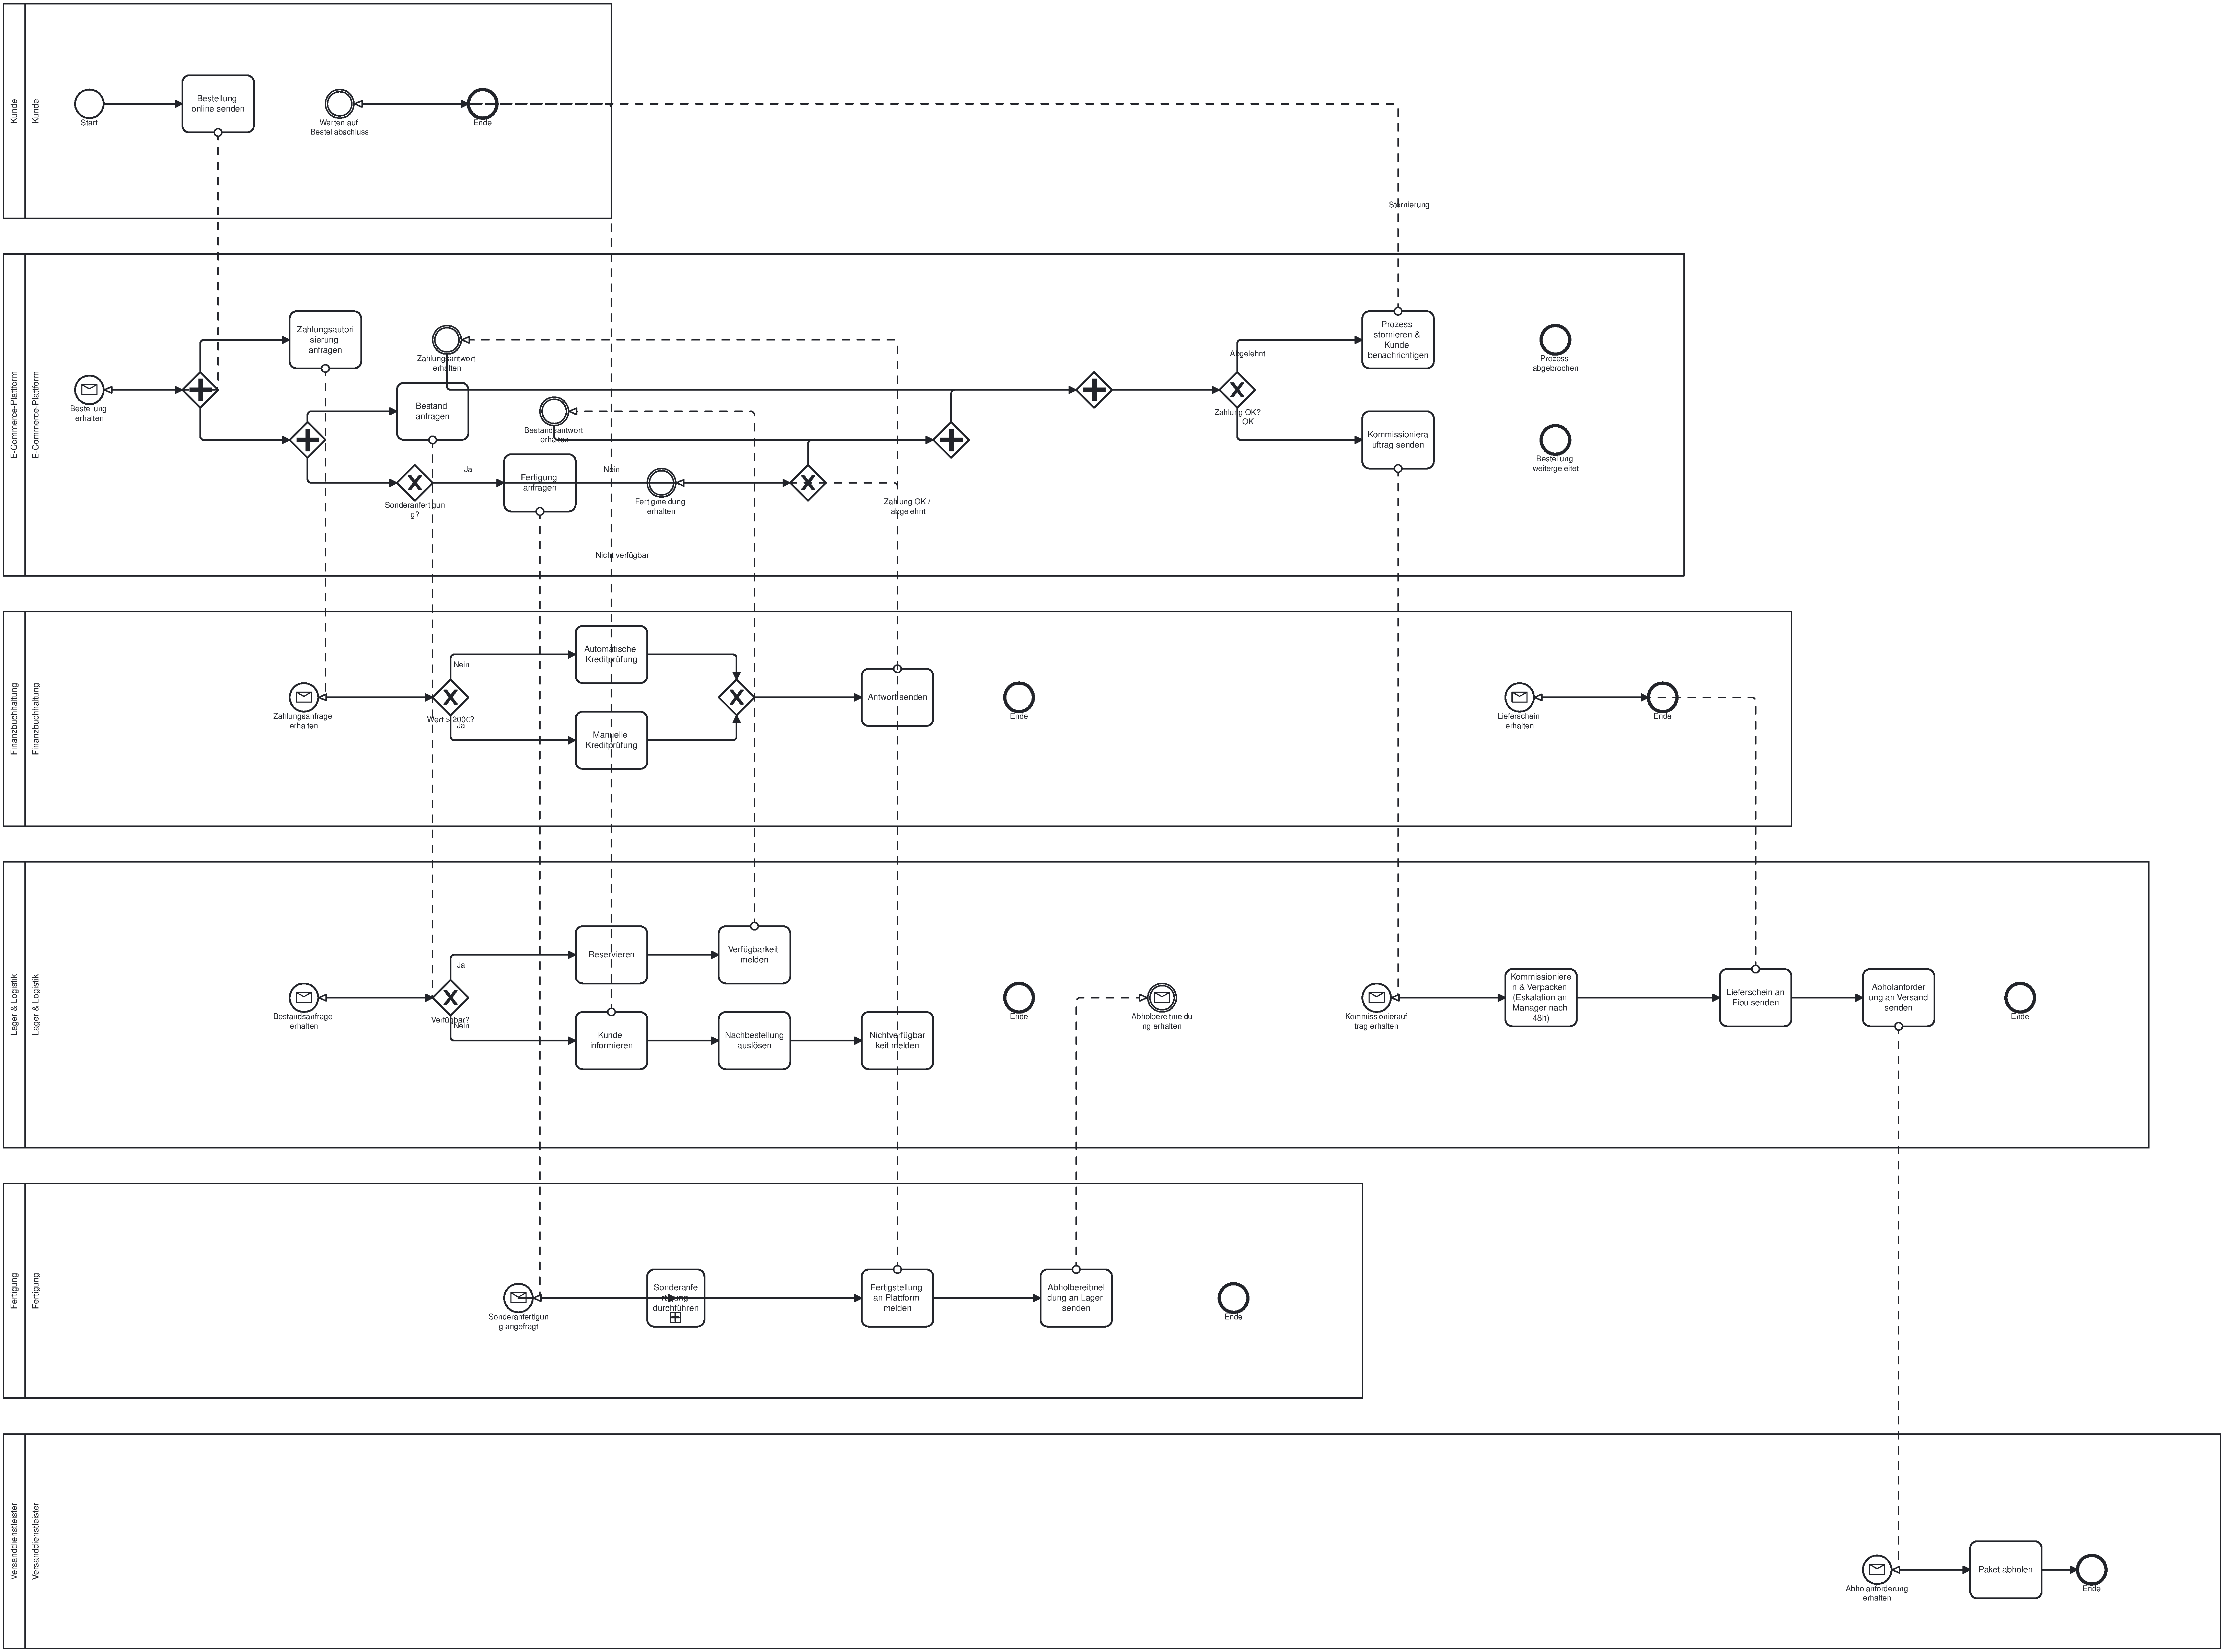
\includegraphics[width=\textwidth]{images/diagrams/gemini-2.5-pro-(json)-9zeuvovk}
    \caption{Diagramm von Gemini 2.5 Pro mit JSON}
    \label{fig:gemini-2-5-pro-json}
\end{figure}

\begin{figure}[!htb]
    \centering
    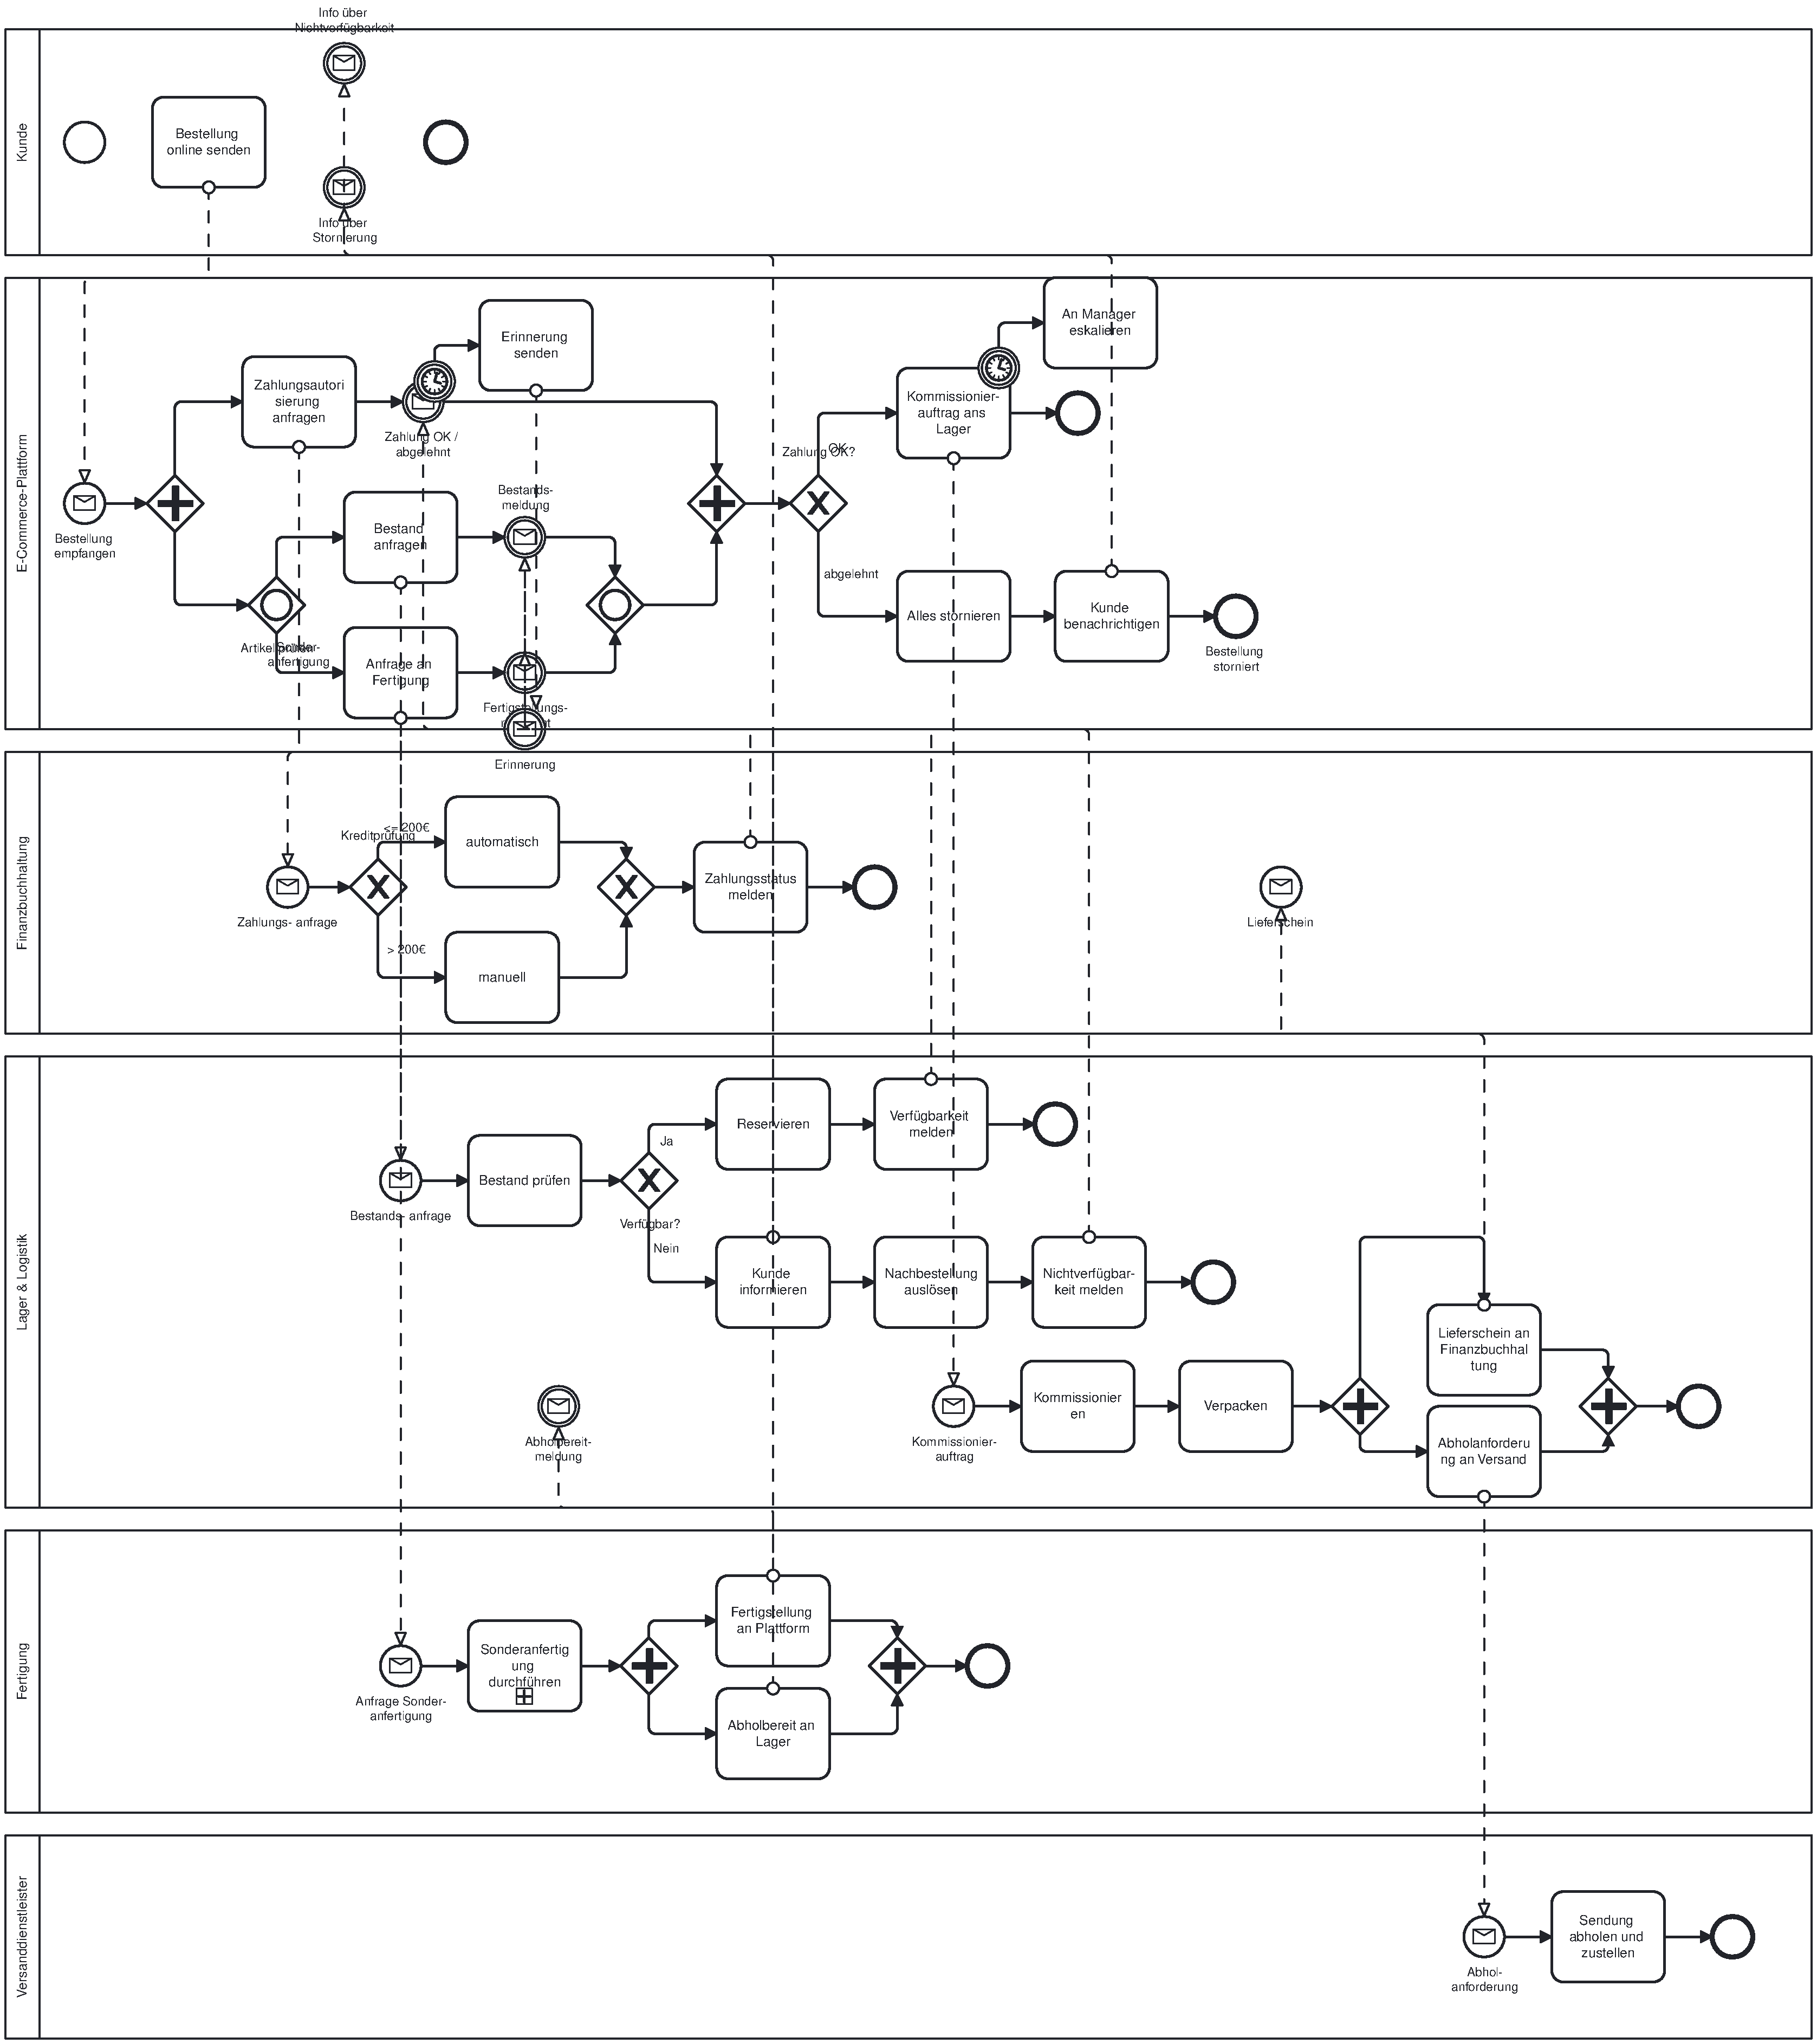
\includegraphics[width=\textwidth]{images/diagrams/gemini-2.5-pro-(xml)-67z0in69}
    \caption{Diagramm von Gemini 2.5 Pro mit XML}
    \label{fig:gemini-2-5-pro-xml}
\end{figure}

\begin{figure}[!htb]
    \centering
    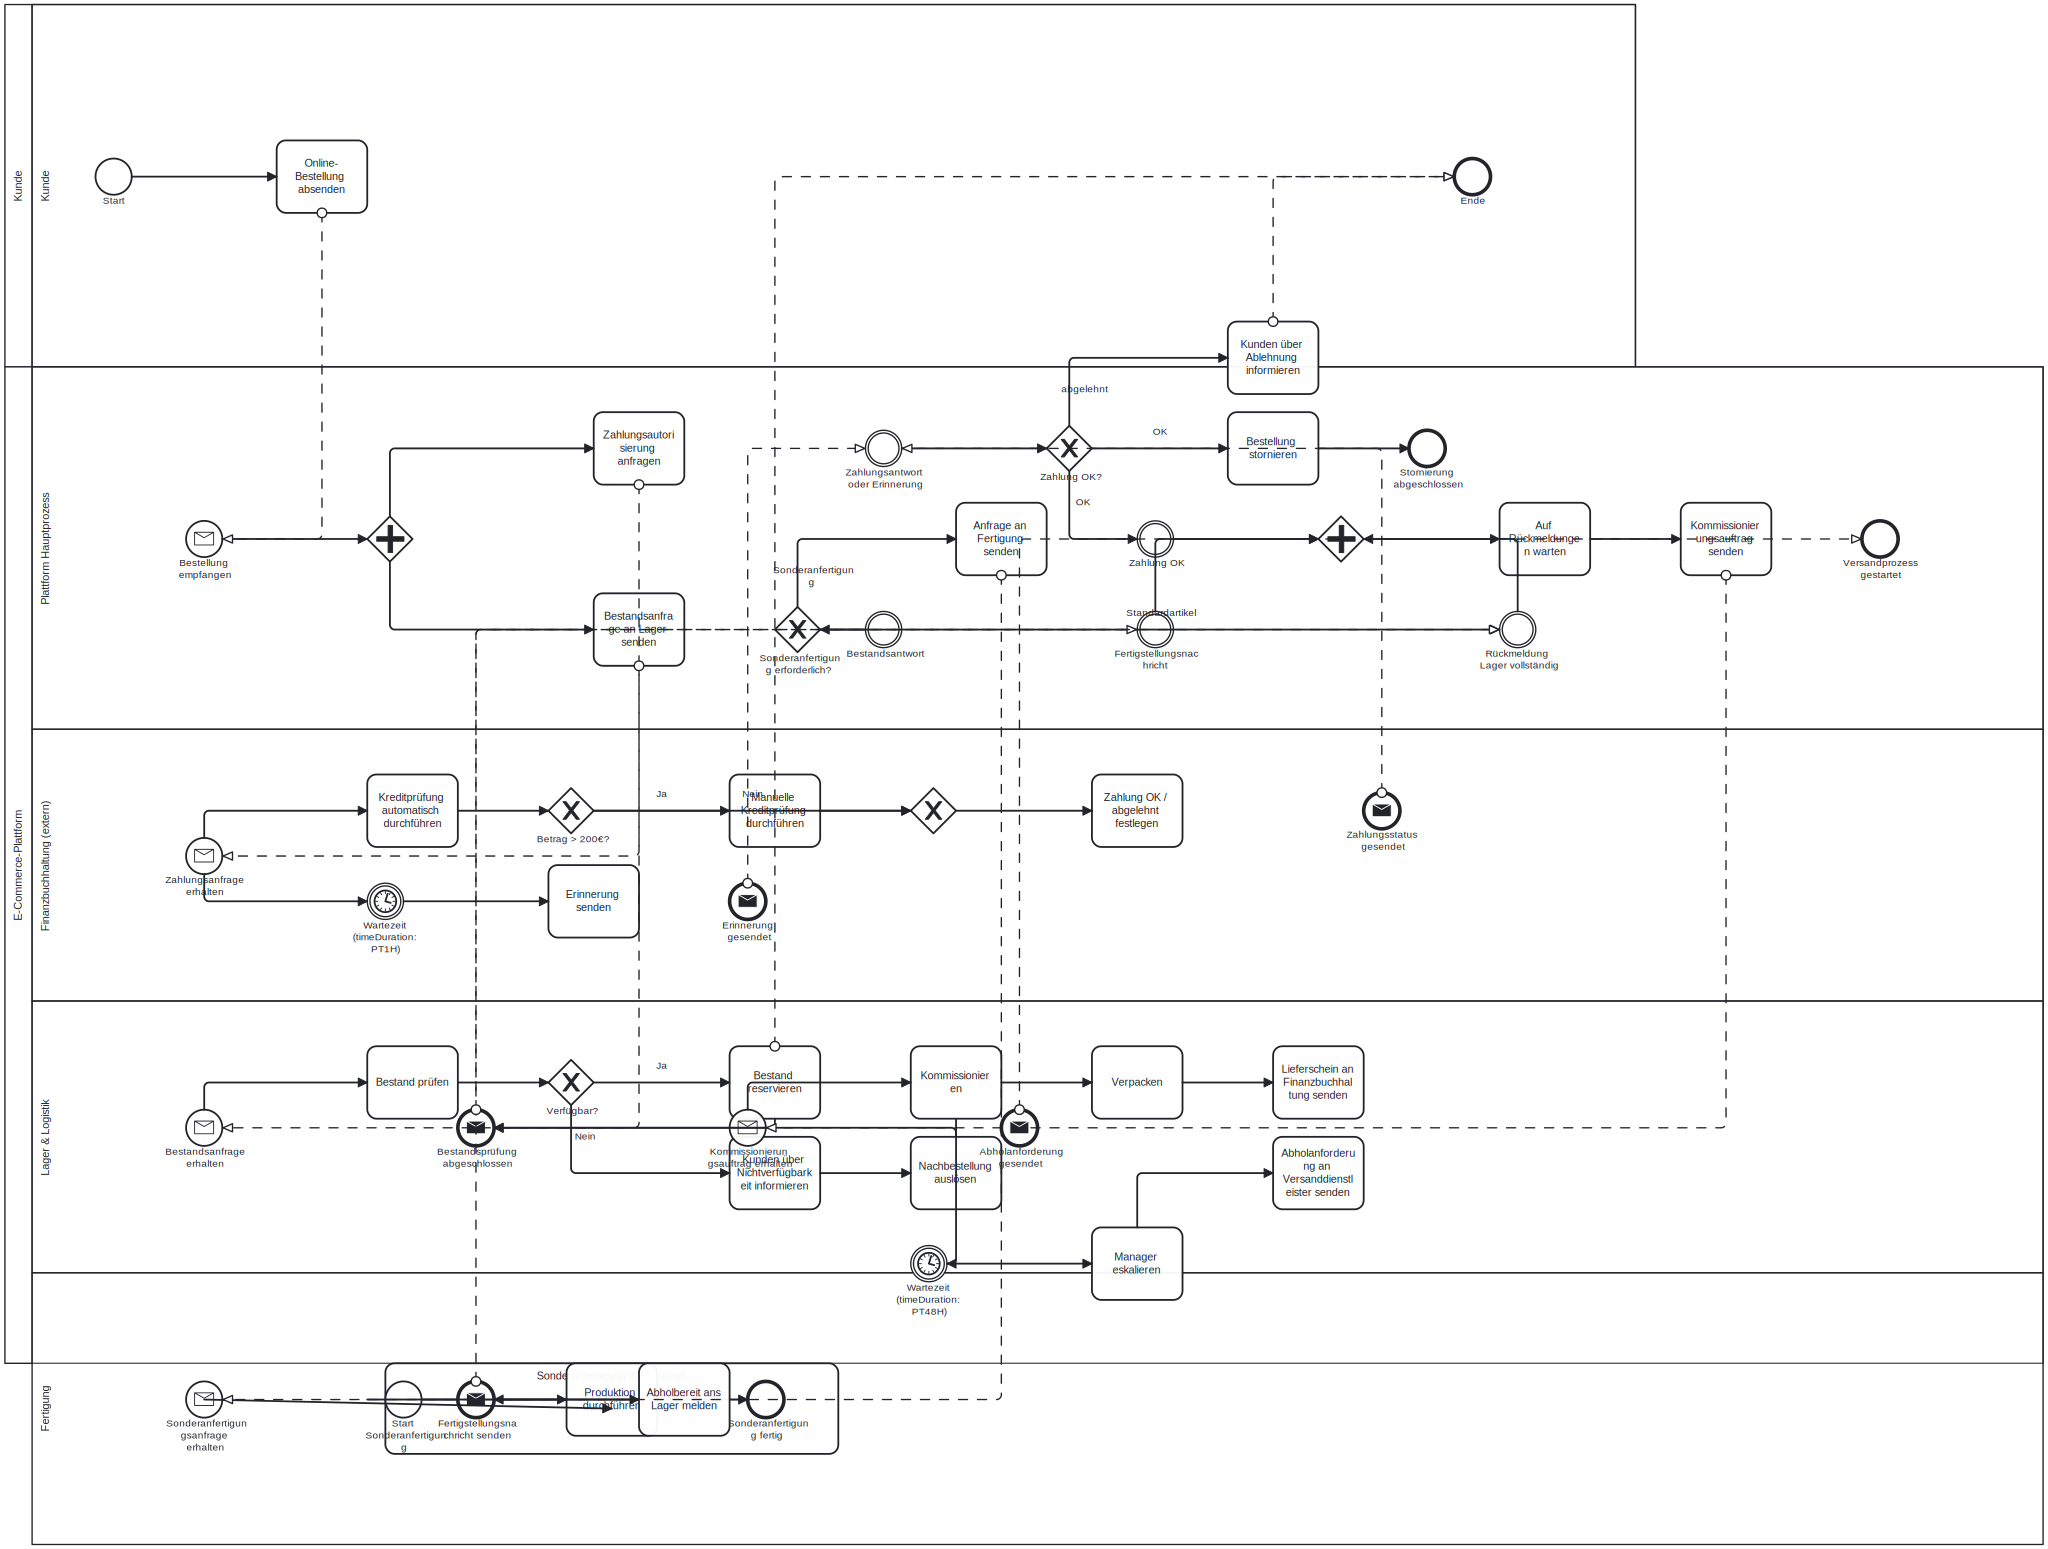
\includegraphics[width=\textwidth]{images/diagrams/gpt-5.1-(json)-ai2w4c2b}
    \caption{Diagramm von ChatGPT 5.1 mit JSON}
    \label{fig:gpt-5-1-json}
\end{figure}

\begin{figure}[!htb]
    \centering
    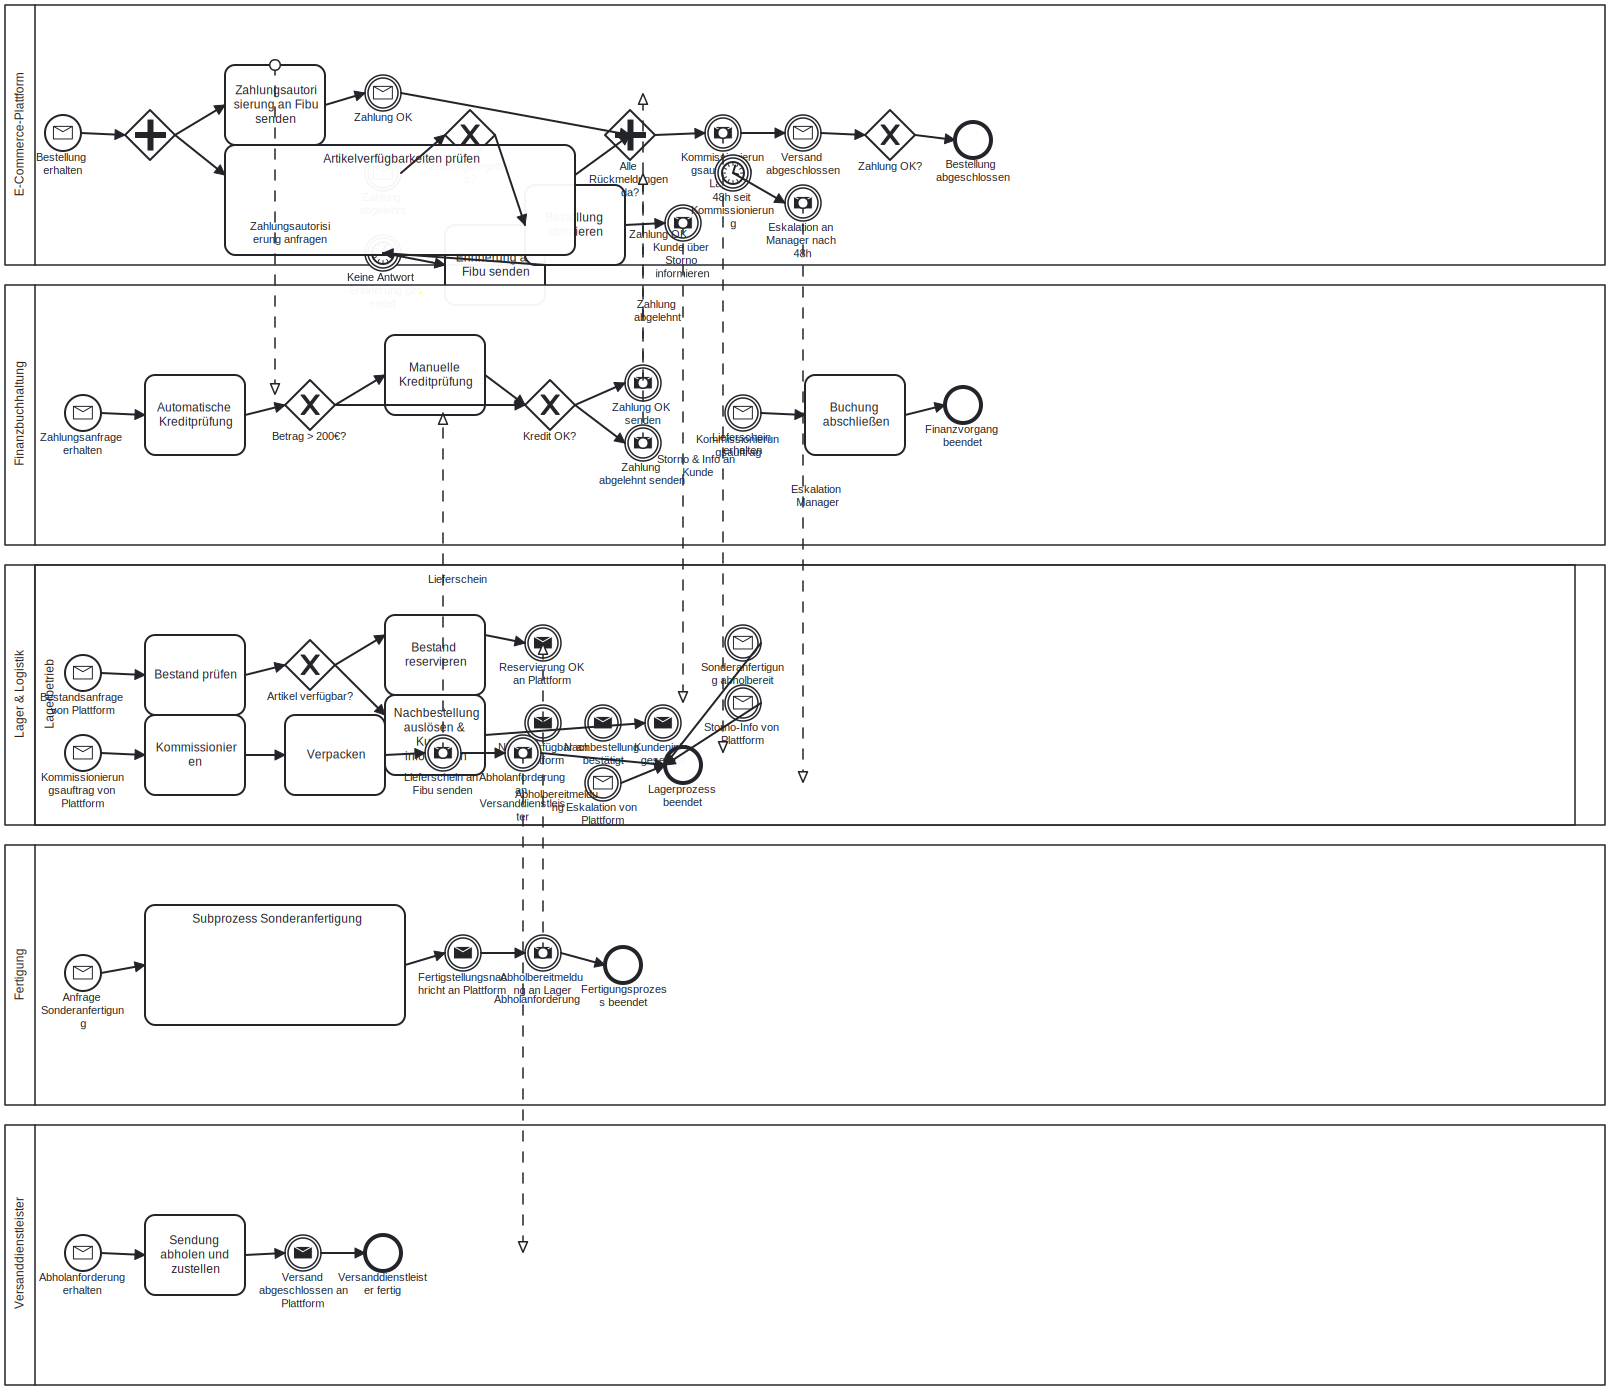
\includegraphics[width=\textwidth]{images/diagrams/gpt-5.1-(xml)-obl5u8o2}
    \caption{Diagramm von ChatGPT 5.1 mit XML}
    \label{fig:gpt-5-1-xml}
\end{figure}

\begin{figure}[!htb]
    \centering
    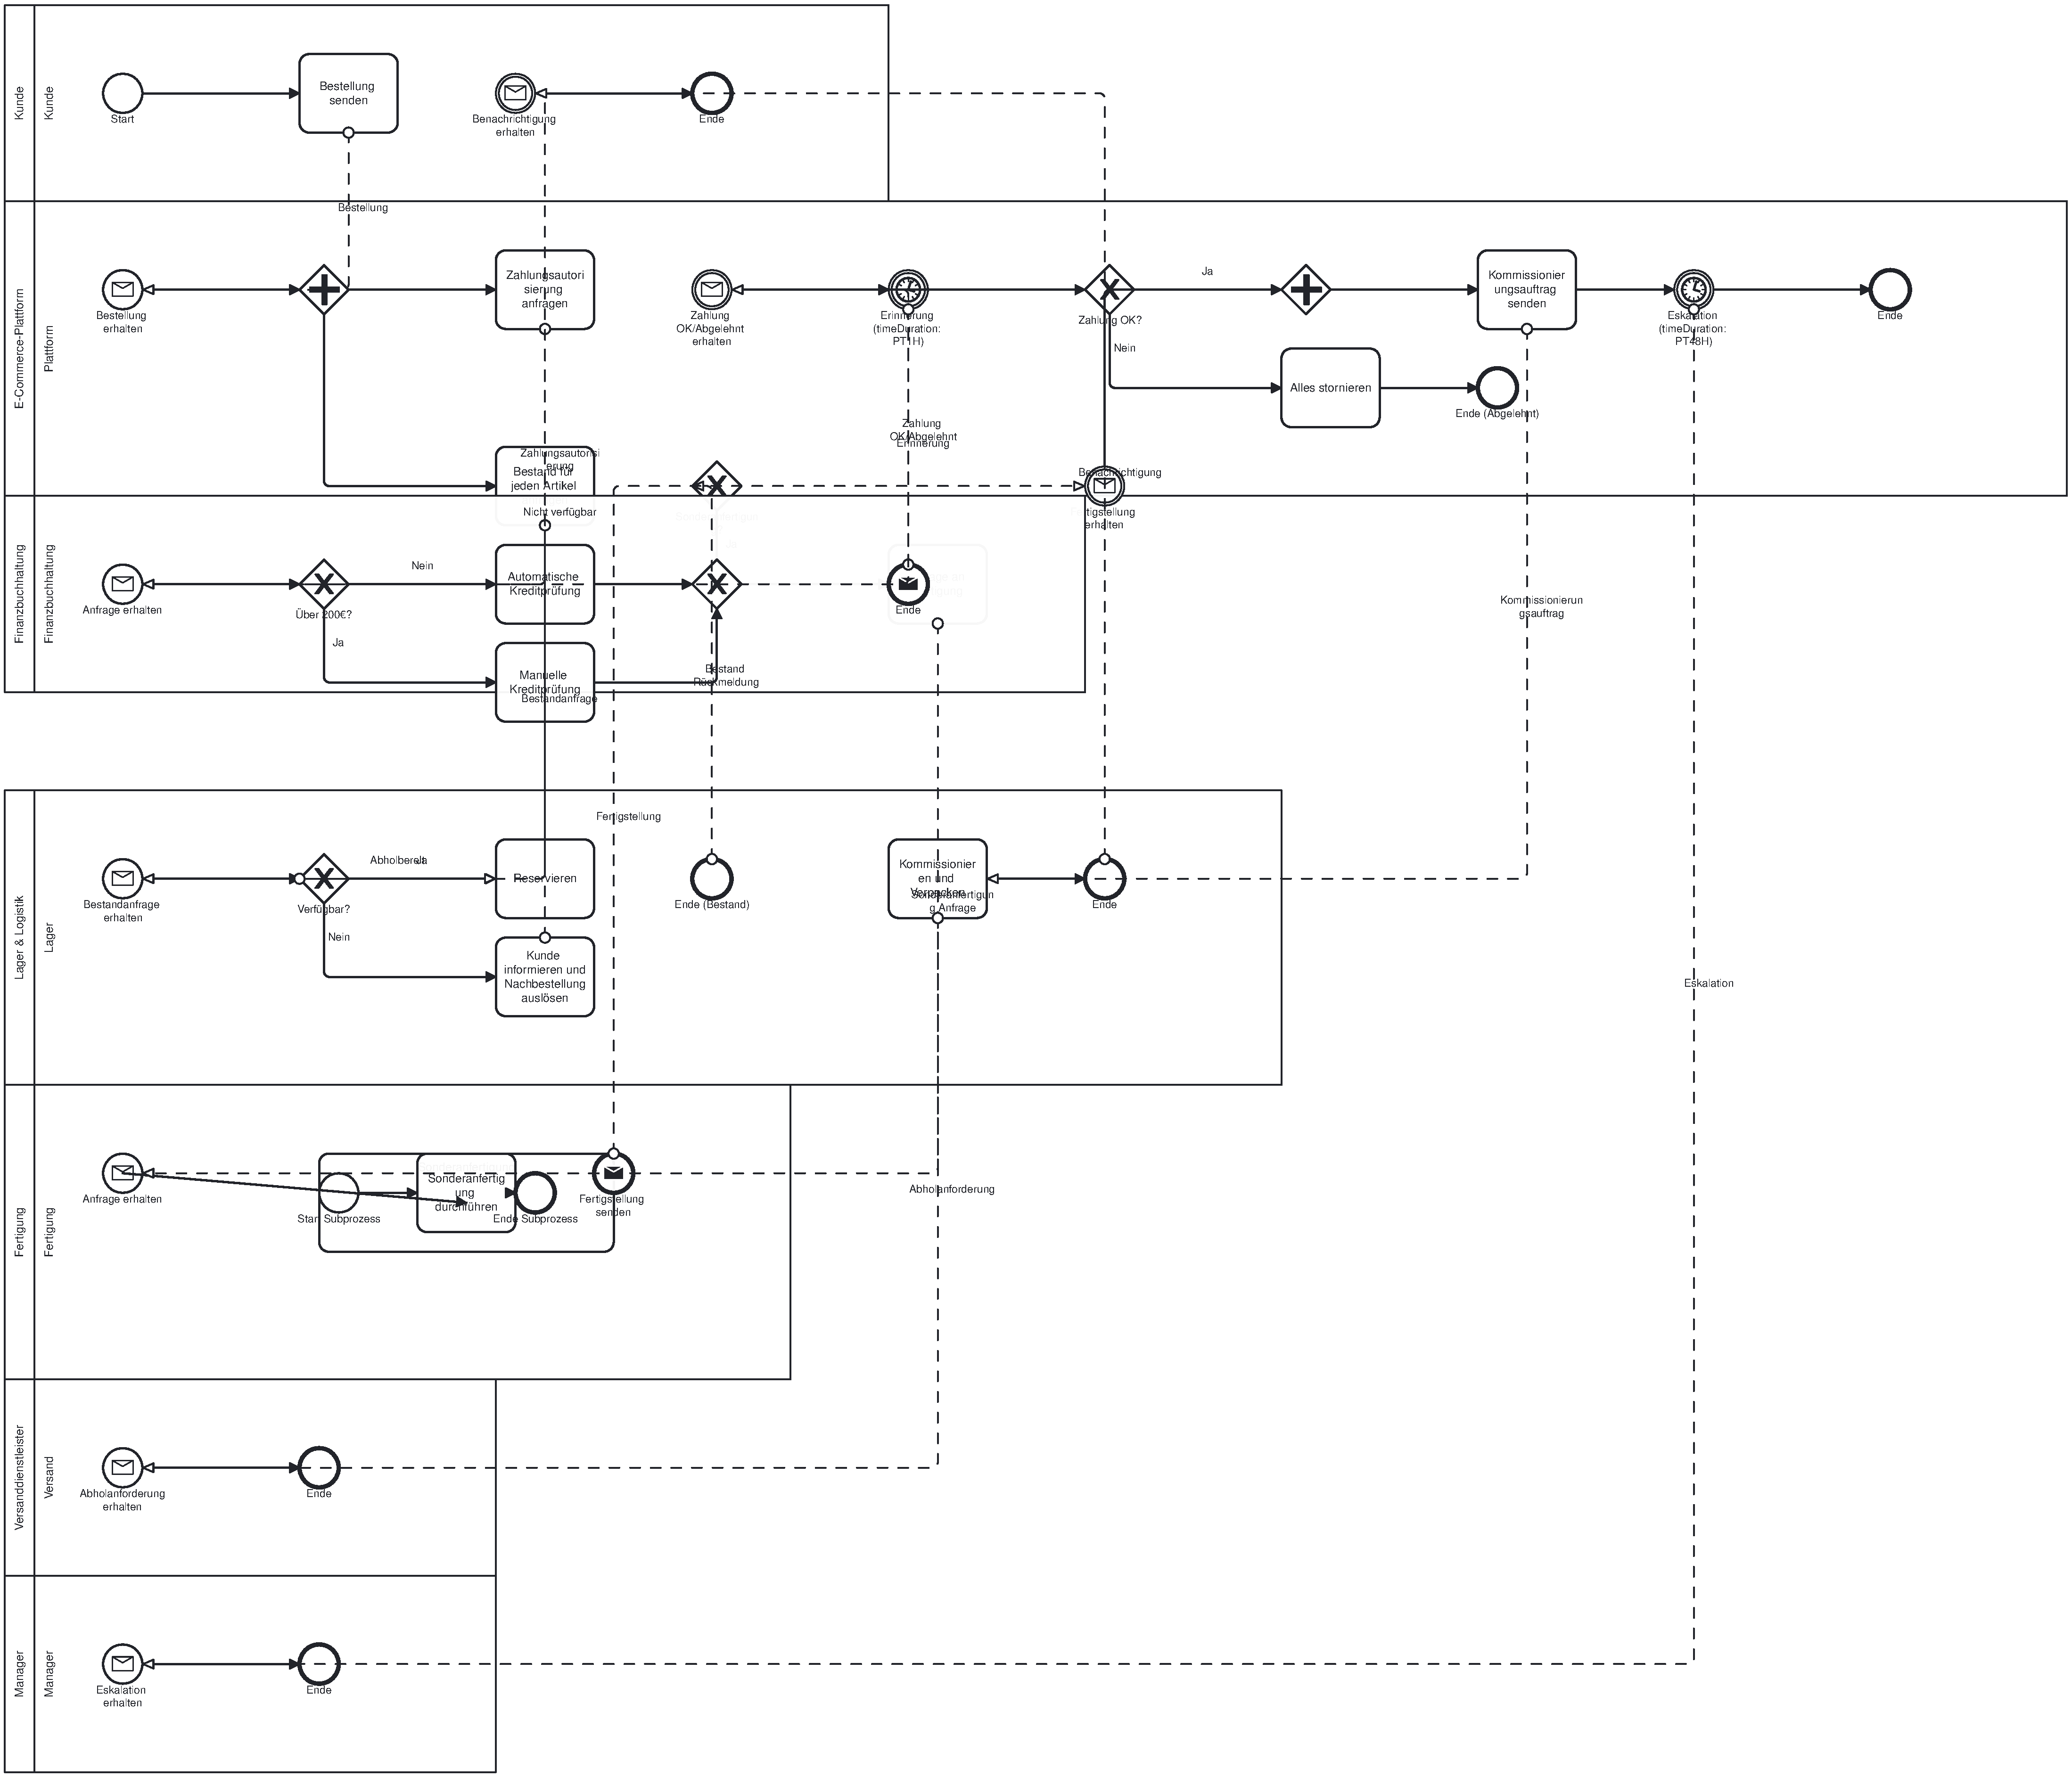
\includegraphics[width=\textwidth]{images/diagrams/grok-4-(json)-0pkdhn37}
    \caption{Diagramm von Grok 4 mit JSON}
    \label{fig:grok-4-json}
\end{figure}

\begin{figure}[!htb]
    \centering
    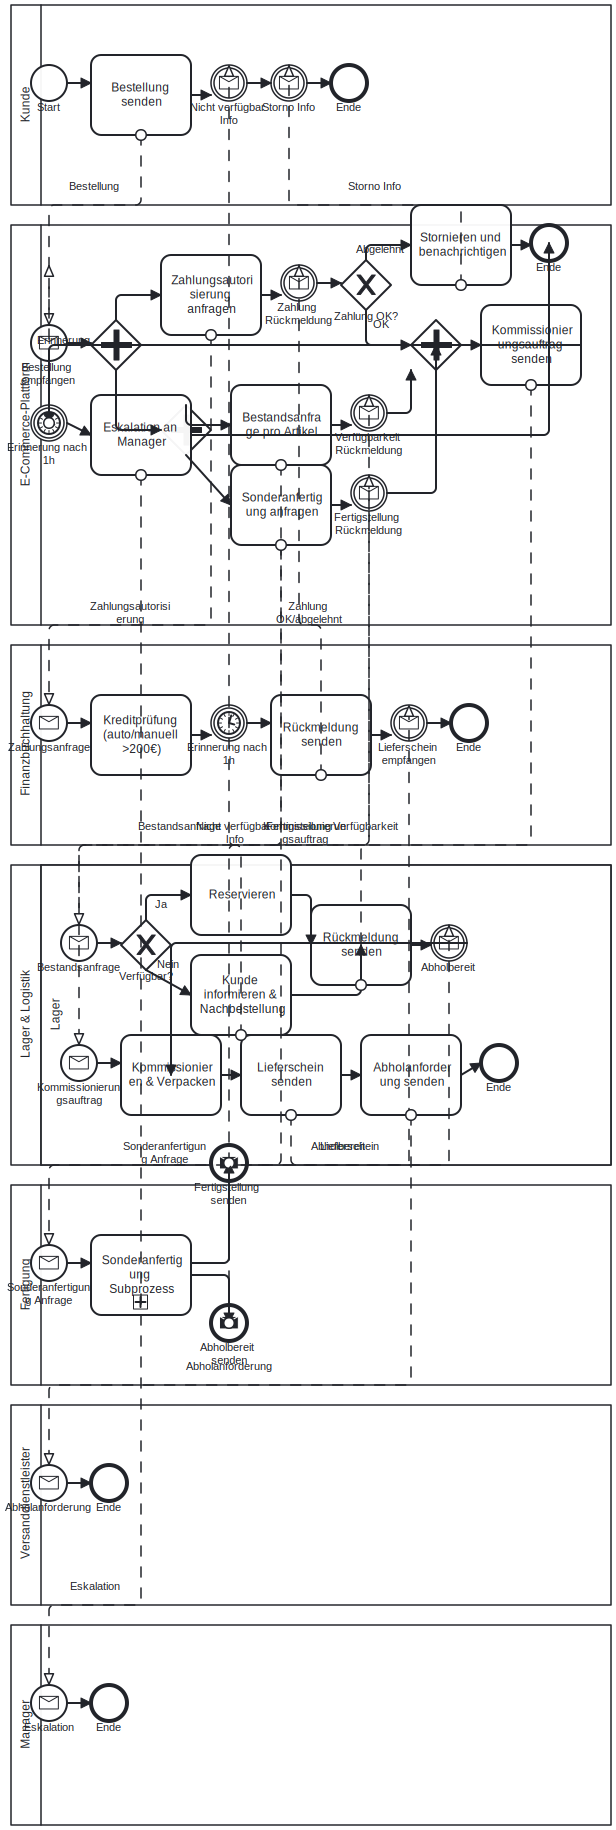
\includegraphics[height=.95\textheight]{images/diagrams/grok-4-(xml)-zyw3qofn}
    \caption{Diagramm von Grok 4 mit XML}
    \label{fig:grok-4-xml}
\end{figure}

\begin{figure}[!htb]
    \centering
    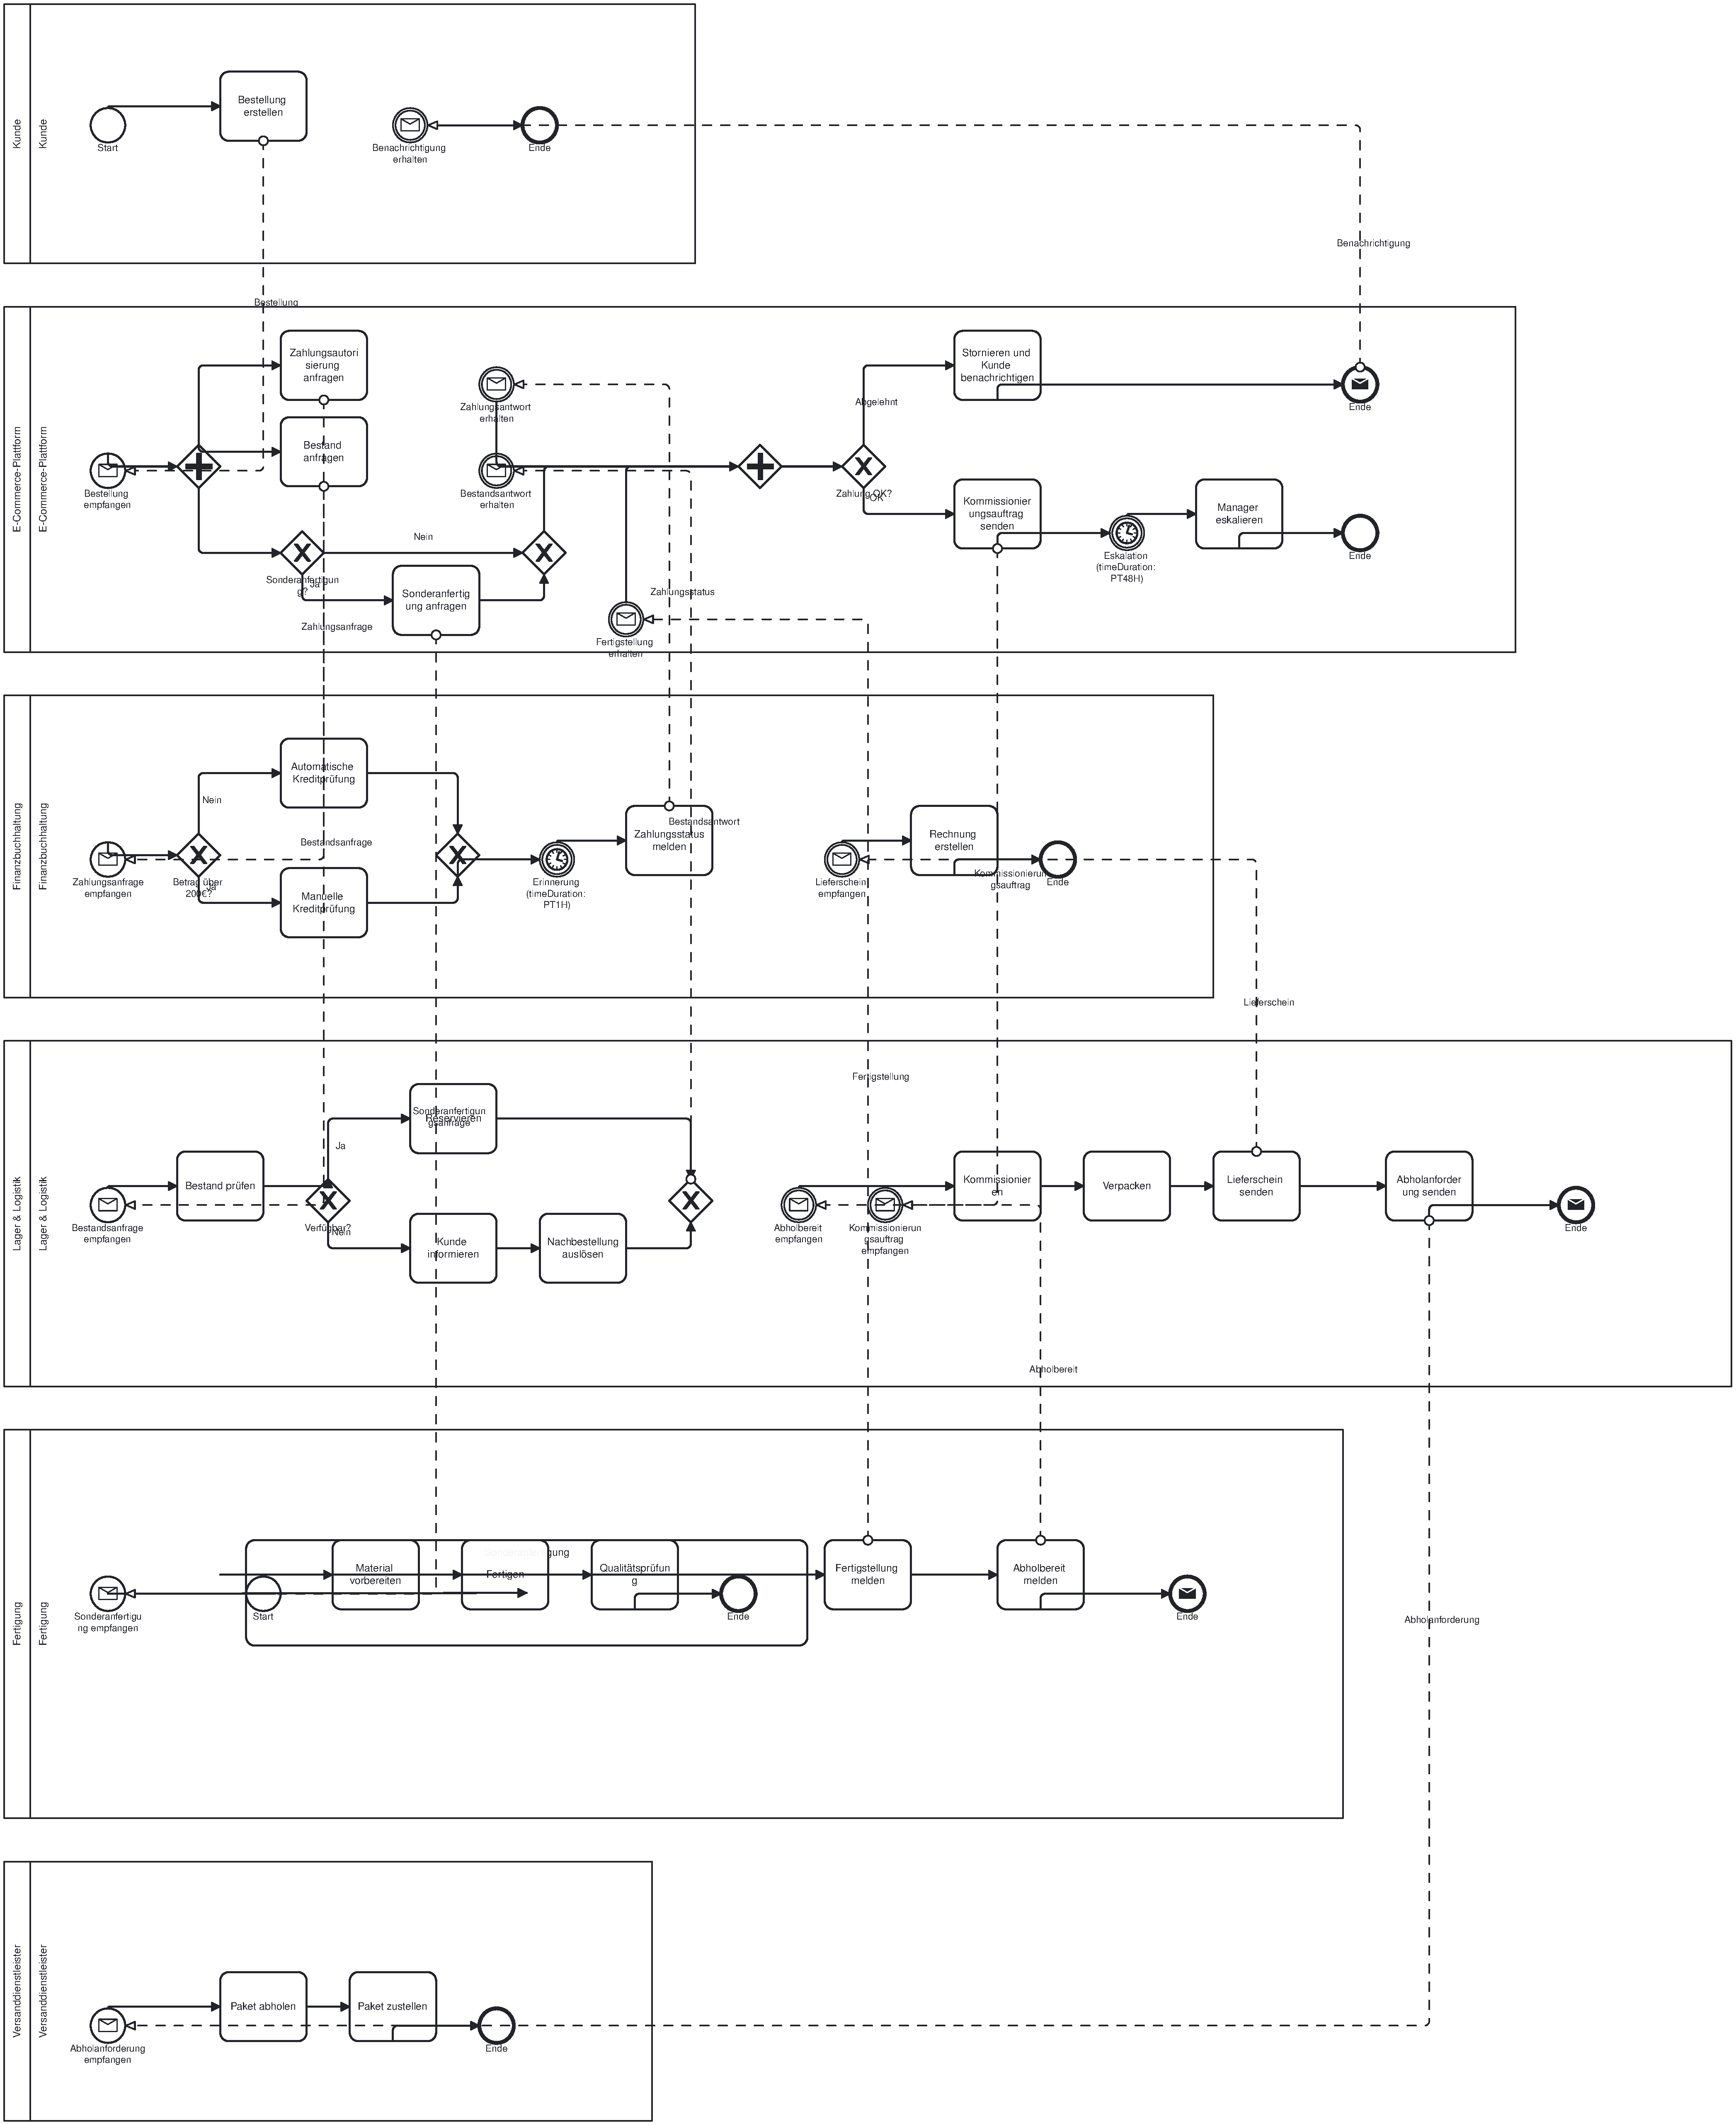
\includegraphics[width=\textwidth]{images/diagrams/claude-opus-4-5-(json)-p0ejrwf2}
    \caption{Diagramm von Claude Opus 4.5 mit JSON}
    \label{fig:claude-opus-4-5-json}
\end{figure}
